% -*- mode: fundamental -*-

% ****************************************************************

\chapter{RISC-V: the Fife pipelined CPU: BSV code}

\markboth{Ch \arabic{chapter}: Fife BSV code (DRAFT)}{\copyrightnotice}

\setcounter{page}{1}
% \renewcommand{\thepage}{\arabic{page}}
\renewcommand{\thepage}{\arabic{chapter}-\arabic{page}}

\label{ch_Fife_code}

% ****************************************************************

\section{Introduction}

In this chapter we study BSV code to implement the principles that
were discussed in the previous chapter.  We repeat
Figure~\ref{Fig_Instr_Exec_w_FIFOs} here, for reference.
\begin{figure}[htbp]
  \centerline{\includegraphics[width=6in,angle=0]{Figures/Fig_Instr_Exec_w_FIFOs}}
  \caption{\label{Fig_Instr_Exec_w_FIFOs_2}Pipelined interpretation of RISC-V instructions (Fig.~\ref{Fig_Instr_Exec} with some annotations)}
\end{figure}

% ****************************************************************

\section{The Fife top-level CPU module}

\label{Sec_Fife_CPU_module}

The code for the top-level Fife CPU module is actually simpler than
the code for the Drum CPU module:

{\small
\begin{Verbatim}[frame=single, numbers=left, label=(In file:src\_Fife/CPU.bsv)]
(* synthesize *)
module mkCPU (CPU_IFC);
   // Pipeline stages
   Fetch_IFC       stage_F          <- mkFetch;
   Decode_IFC      stage_D          <- mkDecode;
   RR_RW_IFC       stage_RR_RW      <- mkRR_RW;
   EX_Control_IFC  stage_EX_Control <- mkEX_Control;  // Branch, JAL, JALR
   EX_Int_IFC      stage_EX_Int     <- mkEX_Int;      // Integer ops
   Retire_IFC      stage_Retire     <- mkRetire;

   // ================================================================
   // Forward flows

   // F->D->RR_RW->Retire
   mkConnection (stage_F.fo_F_to_D,           stage_D.fi_F_to_D);
   mkConnection (stage_D.fo_D_to_RR,          stage_RR_RW.fi_D_to_RR);
   mkConnection (stage_RR_RW.fo_RR_to_Retire, stage_Retire.fi_RR_to_Retire);

   // RR->various EX
   mkConnection (stage_RR_RW.fo_RR_to_Control, stage_EX_Control.fi_RR_to_Control);
   mkConnection (stage_RR_RW.fo_RR_to_EX_IALU, stage_EX_Int.fi_RR_to_EX_IALU);

   // Various EX->Retire
   mkConnection (stage_EX_Control.fo_Control_to_Retire,
		 stage_Retire.fi_Control_to_Retire);
   mkConnection (stage_EX_Int.fo_EX_IALU_to_Retire,
		 stage_Retire.fi_IALU_to_Retire);

   // ================================================================
   // Backward flows

   // F<-RR (redirection)
   mkConnection (stage_Retire.fo_F_from_Retire,  stage_F.fi_F_from_Retire);
   // RR<-RW (writeback/trap/flush)
   mkConnection (stage_Retire.fo_RW_from_Retire, stage_RR_RW.fi_RW_from_Retire);

   // ================================================================
   // INTERFACE

   method Action init (Initial_Params initial_params);
      stage_F.init (initial_params);
      ... and similarly, for all the other stages ...
   endmethod

   interface fo_IMem_req = stage_F.fo_F_to_IMem;
   interface fi_IMem_rsp = stage_D.fi_IMem_to_D;

   interface fo_DMem_S_req    = stage_RR_RW.fo_DMem_S_req;
   interface fi_DMem_S_rsp    = stage_Retire.fi_DMem_S_rsp;
   interface fo_DMem_S_commit = stage_Retire.fo_DMem_S_commit;

   interface fo_DMem_NS_req = stage_Retire.fo_DMem_NS_req;
   interface fi_DMem_NS_rsp = stage_Retire.fi_DMem_NS_rsp;
endmodule
\end{Verbatim}
}

This is practically a direct textual description of
Figure~\ref{Fig_Instr_Exec_w_FIFOs_2}.  The first few lines
instantiate the pipeline stages shown in the figure.  There is no
explicit module corresponding to Execute Memory Ops---the DMem request
is sent out directly from \verb|stage_RR_RW| and the DMem response is
collected directly by \verb|stage_Retire|.

The next several lines make the ``forward-flow'' connections between
modules (left to right in the figure) .  These are followed by lines
making the ``backward-flow'' connections.  All these use the
\verb|mkConnection| module to connect a \verb|FIFOF_O| interface
(producer) to a \verb|FIFOF_I| interface (consumer), which was
discussed in Section~\ref{Sec_connecting_FIFOs}.

In the INTERFACE section, after the \verb|init| method, the next two
lines are the flows of IMem requests from the Fetch stage to memory
and IMem responses from memory to the Decode stage.  These just lift
interfaces from \verb|stage_F| and \verb|stage_D| to the CPU
interface, as is.

The next three lines are for \emph{speculative} DMem access, which we
discussed in Section~\ref{Sec_Store_Buffers}: the flow of DMem
requests from \verb|stage_RR| to memory, the flow of DMem responses
from memory to \verb|stage_Retire|, and the flow of ``commit/discard''
messages from \verb|stage_Retire| to the store-buffer to discharge
STOREs that are waiting in the store-buffer.

The last two lines are for \emph{non-speculative} DMem access, which
we discussed in Section~\ref{Sec_DMem_MMIO}.

Note that the module interface \verb|CPU_IFC| is exactly the same as
in Drum (although Drum has no need for, and does not use the
speculative DMem interfaces).  Thus, in a system context, we can
directly substitute Drum for Fife and vice versa.  Generalizing, we
can develop other CPUs and substitute them, as well.

% ****************************************************************

\section{Fife: the Fetch stage}

\label{Sec_Fife_Fetch_stage}

The Fetch stage module code is shown below.

{\small
\begin{Verbatim}[frame=single, numbers=left, label=(In file:src\_Fife/S1\_Fetch.bsv)]
(* synthesize *)
module mkFetch (Fetch_IFC);
   Reg #(Bool) rg_running <- mkReg (False);

   // Forward out
   FIFOF #(F_to_D)  f_F_to_D    <- mkBypassFIFOF;
   FIFOF #(Mem_Req) f_F_to_IMem <- mkBypassFIFOF;

   // Backward in
   FIFOF #(F_from_Retire) f_F_from_Retire <- mkPipelineFIFOF;

   // inum, PC and epoch registers
   Reg #(Bit #(64))       rg_inum  <- mkReg (0);
   Reg #(Bit #(XLEN))     rg_pc    <- mkReg (0);
   Reg #(Bit #(W_Epoch))  rg_epoch <- mkReg (0);

   // ----------------------------------------------------------------
   // BEHAVIOR

   // Forward flow
   rule rl_Fetch_req (rg_running && (! f_F_from_Retire.notEmpty));
      // Predict next PC
      let pred_pc = rg_pc + 4;

      let y <- fn_F (rg_inum, rg_pc, pred_pc, rg_epoch);
      f_F_to_D.enq (y.to_D);
      f_F_to_IMem.enq (y.mem_req);

      rg_pc   <= pred_pc;
      rg_inum <= rg_inum + 1;
   endrule

   // Backward flow: redirection from Retire
   rule rl_F_from_Retire;
      let x <- pop_o (to_FIFOF_O (f_F_from_Retire));

      rg_pc    <= x.next_pc;
      rg_epoch <= x.next_epoch;
   endrule

   // ----------------------------------------------------------------
   // INTERFACE

   method Action init (Initial_Params initial_params) if (! rg_running);
      ...
      rg_pc      <= initial_params.pc_reset_value;
      rg_running <= True;
   endmethod

   // Forward out
   interface fo_F_to_D    = to_FIFOF_O (f_F_to_D);
   interface fo_F_to_IMem = to_FIFOF_O (f_F_to_IMem);

   // Backward in
   interface fi_F_from_Retire = to_FIFOF_I (f_F_from_Retire);
endmodule
\end{Verbatim}
}

The first section of the module instantiates some registers and FIFOs.

Next, the BEHAVIOR section contains two \emph{rules}, which are the
fundamental dynamic behavior constructs in BSV.  A rule is an infinite
process.  Every rule consists of a \emph{condition} and an
\emph{action}: whenever the condition is true, the action is
performed; we say the rule ``fires'' whenever its condition is
true.\footnote{Topic discussed later in the book: a rule may not fire
even if its condition is true, if it ``conflicts'' with another rule.}

A rule may contain explicit and implicit conditions. In rule
\verb|rl_Fetch_req|, the explicit condition is the expression:

\hm\small \verb|(rg_running && (! f_F_from_Retire.notEmpty))|

Rule \verb|rl_Fetch_req|'s implicit conditions come from the methods
that it invokes, specifically: \verb|f_F_to_D.enq ()| and
\verb|f_F_to_IMem.enq ()|.  Every method has an implicit conditions.
For a FIFO, the \emph{enq()} method's implicit condition is false when
the FIFO is full, {\ie} when it does not contain space to enqueue a
new item.  We also say the method is ``enabled'' when its implicit
condition is true.

In summary, rule \verb|rl_Fetch_req| will fire only when the explicit
condition is true, and when both FIFOs on which it tries to enqueue
are enabled.  When it fires, it performs a composite action that
includes all the actions stated in the rule:

\begin{tightlist}

 \item enqueues into \verb|f_F_to_D| the value of \verb|y.to_D|,

 \item enqueues into \verb|f_F_to_IMem| the value of \verb|y.mem_req|,

 \item writes \verb|pred_pc| into \verb|rg_pc|,

 \item and writes the value of \verb|rg_inum+1| into \verb|rg_inum|.

\end{tightlist}
where \verb|y| is the result of applying \verb|fn_F| to
\verb|rg_inum|, \verb|pred_pc| and \verb|rg_epoch|, where
\verb|pred_pc| is the value of \verb|rg_pc+4.|,

NOTE:
\fbox{\small
\begin{minipage}{5in}

The function {\tt fn\_F()} invoked in rule {\tt rl\_Fetch} is exactly
the same one as {\tt fn\_F()} used in the Fetch step of Drum.

\vspace{1ex}

The types of the messages passed to the Decode stage ({\tt y.to\_D} of
type {\tt F\_to\_D}) and to memory ({\tt y.mem\_req} of type {\tt
Mem\_Req}) are the same as in Drum.

\end{minipage}}

All these actions are semantically \emph{instantaneous} and
\emph{simultaneous}.  Note that when the rule's implicit and explicit
conditions are true, all the actions are peformed; if false, none of
them are performed.  We also say that the rule's composite action is
``atomic''.

In summary, rule \verb|rl_Fetch_req| computes an IMem memory request
from the PC and sends it to memory; it sends auxiliary information to
the Decode stage; and it updates the PC and inum in preparation for
the next Fetch.

Rule \verb|rl_F_from_Retire| receives, in \verb|x|, a redirection
message from the Retire stage, and updates the PC and epoch
accordingly.  This rule has no explicit conditions; its single
implicit condition comes from \verb|f_F_from_Retire|'s implicit
condition that we cannot pop a value from the FIFO if it is empty,
{\ie}, this rule only fires when a redirection message is available.
When it fires, it performs three actions
atomically/instantaneously/simultaneously:
 
\begin{tightlist}

 \item It dequeues \verb|x| from the FIFO \verb|f_F_from_Retire| (the
       dequeue action is inside the \verb|pop_o| function),
 \item It updates \verb|rg_pc| with the new PC in the redirection message,
 \item It updates \verb|rg_epoch| with the new epoch in the redirection message.

\end{tightlist}

Note, \verb|rl_F_from_Retire| updates two registers \verb|rg_pc| and
\verb|rg_epoch| and, \emph{concurrently}, \verb|rl_Fetch| reads both
those registers.  Because rule actions are atomic, we are guaranteed
that \verb|rl_Fetch| will not see inconsitent values in those two
registers, where one has been updated but the other has not yet been
updated.

Finally, the INTERFACE section of the module is simple.  After the
\verb|init| method, we simply lift the FIFO interfaces to the
\verb|mkFetch| interface.

% ****************************************************************

\section{Fife: the Decode stage}

The Decode stage module code is shown below.

\label{Sec_Fife_Decode_stage}

{\small
\begin{Verbatim}[frame=single, numbers=left, label=(In file:src\_Fife/S2\_Decode.bsv)]
(* synthesize *)
module mkDecode (Decode_IFC);
   // Forward flows in
   // Depth should be > F=>IMem=>D path latency
   FIFOF #(F_to_D)  f_F_to_D    <- mkSizedFIFOF (4);
   FIFOF #(Mem_Rsp) f_IMem_to_D <- mkPipelineFIFOF;

   // Forward flow out
   FIFOF #(D_to_RR) f_D_to_RR   <- mkBypassFIFOF;

   // ================================================================
   // Functionality

   rule rl_Decode;
      F_to_D  x        <- pop_o (to_FIFOF_O (f_F_to_D));
      Mem_Rsp rsp_IMem <- pop_o (to_FIFOF_O (f_IMem_to_D));

      D_to_RR y <- fn_D (x, rsp_IMem);

      f_D_to_RR.enq (y);
   endrule

   // ================================================================
   // INTERFACE

   method Action init (Initial_Params initial_params);
      ...
   endmethod

   // Forward flows in
   interface fi_F_to_D    = to_FIFOF_I (f_F_to_D);
   interface fi_IMem_to_D = to_FIFOF_I (f_IMem_to_D);
   // Forward flows out
   interface fo_D_to_RR = to_FIFOF_O (f_D_to_RR);
endmodule
\end{Verbatim}
}

The first section instantiates FIFOs for incoming and outgoing flows.

The single rule \verb|rl_Decode|'s implicit conditions will make it
wait for both incoming FIFOs \verb|f_F_to_D| and \verb|f_IMem_to_D| to
be non-empty.  When the rule fires, it:

\begin{tightlist}
 \item pops \verb|x| and \verb|rsp_Mem| from the two FIFOs, respectively,

 \item applies function \verb|fn_D()| to those values (this is the
       \emph{same} \verb|fn_D()| that was used in the Decode step of
       Drum), and

 \item sends the result on to the Register-Read stage.
\end{tightlist}

The INTERFACE section is again straightforward, just lifting the FIFO
interfaces to this module's interface.

% ****************************************************************

\section{Fife: RR-RW module (Register-Read, Dispatch, Register-Write)}

\label{Sec_Fife_RR_RW_module}

The next module (``RR-RW'') contains the register file and the
scoreboard, and performs several functions. In the forward flow
(``Register-Read and Dispatch'' stage):

\begin{tightlist}

  \item stall (wait) if the instruction has rs1, rs2 or rd, and these
        are busy according to the scoreboard;

  \item read rs1 and rs2 registers (if needed) for the current instruction;

  \item set the scoreboard for rd to 1, meaning ``busy'' (if the
        instruction has an rd);

  \item use the information from the Decode stage to dispatch to the
        Execute pipes.  We always (for every instruction) send an
        execution tag and additional information on the direct path to
        the Retire stage.  We possibly send information into one of
        the following Execute pipes:

  \begin{tightlist}
    \item to Execute Control stage, or
    \item to Execute Control stage, or
    \item to memory (a DMem request).
  \end{tightlist}

\end{tightlist}

In the backward flow (``Register-Write stage''), it receives messages
from the Retire stage to release scoreboard reservations (for
instructions that have retired or aborted due to mispredictions or
traps) and to write-back rd values of retired instructions.

% ================================================================

\subsection{BSV: Vectors for the Scoreboard}

\label{Sec_Fife_Scoreboard}

\index{BSV!vector@{\tt vector}!library data type}

In Section~\ref{Sec_Scoreboards} we discussed the general principles
of a scoreboard, and described it as an array of 1-bit values.  In BSV
the following type is used to represent an array of $n$ items, each of
which is of type $t$:

\begin{tabbing}\small\tt
\hmm Vector \#(n, t);
\end{tabbing}

Note: in order to use this type in any BSV code file, the file must
import the \verb|Vector| library:

\begin{tabbing}\small\tt
\hmm import Vector :: *;
\end{tabbing}

So, we can define a \verb|Scoreboard| type as follows:
\begin{tabbing}\small\tt
\hmm typedef  Vector \#(32, Bit \#(1))  Scoreboard;
\end{tabbing}

\index{BSV!replicate@{\tt replicate} {\tt vector} library function to create a vector value}
\index{BSV!vector@{\tt vector}!library {\tt replicate} function}

The BSV Vector-library function:

\begin{tabbing}\small\tt
\hmm replicate (v)
\end{tabbing}

creates a value of type \verb|Vector #(n, t)| where $n$ is inferred
from the context and \verb|v| has the type $t$.  All $n$ items in the
value are equal to \verb|v|.  Thus, we can instantiate a scoreboard
like this, where all the vector elements are initialized to 0:

\begin{tabbing}\small\tt
\hmm Reg \#(Scoreboard) rg\_scoreboard <- mkReg (replicate (0));
\end{tabbing}

\index{BSV!vector@{\tt vector}!of {\tt n} bits \emph{vs.} {\tt Bit\#(n)}}
\index{BSV!vector@{\tt vector}!representation in bits}

In hardware, a \verb|Vector#(32,Bit#(1))| value occupies exactly 32
bits, {\ie} the size of the vector times the size of each element.
So, why not use \verb|Bit #(32)| instead?  It's a matter of
programming taste:

\begin{tightlist}

  \item The same syntax \verb|v[j]| works both for bit-selection from
        \verb|Bit#(n)| and \verb|Vector#(n,Bit#(1))|.

  \item With \verb|Bit#(n)|, a $j^{th}$ bit can also be selected using
        shift-and-mask operations: \verb|((v >> j) & 1)|.

  \item The $j^{th}$ bit of \verb|Vector#(n,Bit#(1))| can be updated
        using simple assignment \\
	\hmm \verb|v [j] = new_value;|

  \item The $j^{th}$ bit of \verb|Bit#(n)| can be updated using shift
        and mask operations: \\
	\hmm \verb'(v | (1 << j))' to set the $j^{th}$ bit to 1, and \\
	\hmm \verb|(v & (~ (1 << j)))| to resset the $j^{th}$ bit to 0

\end{tightlist}

We can convert a \verb|Vector #(32, Bit #(1))| value into a \verb|Bit#(32)| value with:

\hmm \verb|pack (v)|

and we can convert a \verb|Bit#(32)| value into a \verb|Vector #(32, Bit #(1))| value with:

\hmm \verb|unpack (v)|

% ================================================================

\subsection{The RR-RW module}

\label{Sec_RR_RW_module}

The RR-RW module code is shown below (except we elide the BEHAVIOR
rules, which we will discuss shortly.

{\small
\begin{Verbatim}[frame=single, numbers=left, label=(In file:src\_Fife/S3\_RR\_RW.bsv)]
(* synthesize *)
module mkRR_RW (RR_RW_IFC);
   // Forward in
   FIFOF #(D_to_RR) f_D_to_RR <- mkPipelineFIFOF;

   // Forward out
   FIFOF #(RR_to_Retire)  f_RR_to_Retire  <- mkBypassFIFOF;  // Direct
   FIFOF #(RR_to_Control) f_RR_to_Control <- mkBypassFIFOF;  // Control pipe
   FIFOF #(RR_to_EX)      f_RR_to_EX_IALU <- mkBypassFIFOF;  // Integer pipe
   FIFOF #(Mem_Req)       f_DMem_S_req    <- mkBypassFIFOF;  // DMem pipe

   // Backward in
   FIFOF #(RW_from_Retire) f_RW_from_Retire <- mkPipelineFIFOF;

   // The integer register file (GPRs)
   RISCV_GPRs_IFC #(XLEN)  gprs <- mkRISCV_GPRs;

   // Scoreboard for GPRs
   Reg #(Scoreboard) rg_scoreboard <- mkReg (replicate (0));

   // ================================================================
   // BEHAVIOR

   ... (to be discussed shortly) ...

   // ================================================================
   // INTERFACE

   method Action init (Initial_Params initial_params);
      ...
   endmethod

   // Forward in
   interface fi_D_to_RR = to_FIFOF_I (f_D_to_RR);

   // Forward out
   interface fo_RR_to_Retire  = to_FIFOF_O (f_RR_to_Retire);
   interface fo_RR_to_Control = to_FIFOF_O (f_RR_to_Control);
   interface fo_RR_to_EX_IALU = to_FIFOF_O (f_RR_to_EX_IALU);
   interface fo_DMem_S_req    = to_FIFOF_O (f_DMem_S_req);

   // Backward in
   interface fi_RW_from_Retire = to_FIFOF_I (f_RW_from_Retire);
endmodule
\end{Verbatim}
}

The first section instantiates FIFOs {\tt f\_XXX} for all the forward
and backward flows, and instantiates the register file \verb|gprs| and
the \verb|scoreboard|.

The final INTERFACE section, after the \verb|init| method, simply
lists the FIFO interfaces to this module's interface.

The BEHAVIOR section contains two rules, one for the forward flow
(Register-Read and Dispatch) and one for the backward flow
(Register-Write).  The forward-flow rule is shown below:

{\small
\begin{Verbatim}[frame=single, numbers=left, label=(In file:src\_Fife/S3\_RR\_RW.bsv)]
   rule rl_RR_Dispatch;
      let x = f_D_to_RR.first;

      let instr   = x.instr;
      let opclass = x.opclass;
      let rs1     = instr_rs1 (instr);
      let rs2     = instr_rs2 (instr);
      let rd      = instr_rd  (instr);

      let scoreboard = rg_scoreboard;
      let busy_rs1   = (x.has_rs1 && scoreboard [rs1]);
      let busy_rs2   = (x.has_rs2 && scoreboard [rs2]);
      let busy_rd    = (x.has_rd  && scoreboard [rd]);
      Bool stall     = (busy_rs1 || busy_rs2 || busy_rd);

      if (stall) begin
         // no action
      end
      else begin
	 // Not stalled; proceed
	 f_D_to_RR.deq;

	 // Read GPRs
	 let rs1_val = gprs.read_rs1 (rs1);
	 let rs2_val = gprs.read_rs2 (rs2);

	 // Dispatch to one of the next-stage pipes
	 Result_Dispatch y <- fn_Dispatch (rg_flog, x, rs1_val, rs2_val);

	 // Direct to Retire
	 f_RR_to_Retire.enq (y.to_Retire);

	 // Dispatch
	 if (y.to_Retire.exec_tag == EXEC_TAG_RETIRE) begin
	    // no further action
	 end
	 else begin
	    // Update scoreboard for RD
	    if (x.has_rd) begin
	       scoreboard [rd] = 1;
	       rg_scoreboard <= scoreboard;
	    end

	    // Forward info to appropriate Execute pipe
	    if (y.to_Retire.exec_tag == EXEC_TAG_CONTROL)
	       f_RR_to_Control.enq (y.to_Control);

	    else if (y.to_Retire.exec_tag == EXEC_TAG_IALU)
	       f_RR_to_EX_IALU.enq (y.to_EX);

	    else if (y.to_Retire.exec_tag == EXEC_TAG_DMEM) begin
	       Mem_Req mem_req <- fn_DMem_Req (rg_flog, y.to_EX);
	       f_DMem_S_req.enq (mem_req);
	    end
	    else begin
	       $display ("    -> IMPOSSIBLE");
	       $finish (1);
	    end
	 end
      end
   endrule
\end{Verbatim}
}

In line 2, we observe the first element in the \verb|f_D_to_RR| FIFO.
Note, we observe it non-destructively, {\ie} \emph{we do not dequeue}
it from the FIFO.  This is because, if we must stall, it needs to be
available the next time the rule fires.

The next several lines compute the stall condition by checking the
scoreboard for whether rs1, rs2 or rd are busy (if the instruction has
rs1, rs2 or rd, respectively).

If we stall, the rule takes no action; everything will be retried the
next time it fires.  If we do not stall, then we dequeue the
\verb|f_D_to_RR| FIFO.  We read values of the rs1 and rs2 registers.
Note, if the instruction does not have an rs1 or rs2, here we will be
reading some random registers according to the bits that happen to be
in the rs1 and rs2 bit-positions in the instruction.  This does not
matter; in the Execute stage each instruction only \emph{uses} these
values if the instruction has an rs1 and/or rs2.

Next, we apply the function \verb|fn_Dispatch| (it was discussed in
Section~\ref{Sec_fn_Dispatch}, and is the same one we use in Drum) to
the inputs, which computes \verb|y|, containing the structs to be sent
on the direct path (\verb|y.to_Retire|), to Execute Control
(\verb|y.to_Control|), and to Execute Int and Execute DMem
(\verb|y.toEX|).

We enqueue \verb|y.to_Retire| on the direct flow (FIFO
\verb|f_RR_to_Retire|).  If the execution tag is not
\verb|EXEC_TAG_RETIRE|, we will be sending the instruction into the
one of the Execute pipes (Execute Control, Execute Integer, or DMem).
If the instruction has an rd, we mark it on the scoreboard, and send
the instruction into the appropriate pipe.

% ----------------
\hdivider

\Exercise

Consider this hypothetical scenario: suppose the \verb|stall|
condition is false.  Then, we need to dequeue \verb|f_D_to_RR| and do
one or more enqueues into \verb|f_RR_to_Retire| and
\verb|f_RR_to_Control|, \verb|f_RR_to_EX_IALU| or
\verb|f_DMem_S_req.enq|.  Is it possible that we perform the dequeue
and then are unable to perform the enqueue(s) because the
corresponding output FIFO happens to be full?

\emph{Hint:} Remember the definition of rule atomicity where a rule
only fires if the implicit conditions on \emph{all} the methods it
invokes are true.

\Exercise

Write a boolean expression representing the overall firing condition
for the rule.  Briefly: all FIFO-modifying actions (dequeue, enqueue)
have implicit conditions, but for each FIFO, that condition is only
relevant if the conditions on the surrounding if-then-else's select
that action.

\Exercise

When debugging the implementation, it is useful to know if, due to
some coding mistake, rule \verb|rl_RR_Dispatch| is stalled forever.
For example, for some instruction with an rd, if the Retire stage did
not send back the rd's scoreboard-release, that register will be
forever ``busy''.

Add a register to count consecutive stalls, initially 0.  In the rule,
whenever we successfully dispatch an instruction, reset the counter to
0.  Whenever we stall, increment the stall counter, and if the
stall-counter reaches some chosen threshold value, prints debugging
messages and executes \verb|$finish| to terminate simulation.

\Endexercise

Here is the code for rule \verb|rl_RW_from_Retire| For the backward
flow.

{\small
\begin{Verbatim}[frame=single, numbers=left, label=(In file:src\_Fife/S3\_RR\_RW.bsv)]
   rule rl_RW_from_Retire;
      let x <- pop_o (to_FIFOF_O (f_RW_from_Retire));

      Scoreboard scoreboard = rg_scoreboard;
      scoreboard [x.rd] = 0;
      rg_scoreboard <= scoreboard;

      if (x.commit)
	 gprs.write_rd (x.rd, x.data);
   endrule
\end{Verbatim}
}

We pop the message \verb|x| from the \verb|f_RW_from_Retire| FIFO.  We
perform its specified scoreboard-release for register rd.  If the rd
value is to be committed, we write it into GPR [rd].

% ****************************************************************

\section{Fife: the Execute Control stage}

\label{Sec_Fife_Control_stage}

The code for the Execute Control stage is shown below:

{\small
\begin{Verbatim}[frame=single, numbers=left, label=(In file:src\_Fife/S4\_EX\_Control.bsv)]
(* synthesize *)
module mkEX_Control (EX_Control_IFC);
   // Forward in
   FIFOF #(RR_to_Control)      f_RR_to_Control      <- mkPipelineFIFOF;
   // Forward out
   FIFOF #(Control_to_Retire)  f_Control_to_Retire  <- mkBypassFIFOF;

   // ================================================================
   // BEHAVIOR

   rule rl_Control;
      let x <- pop_o (to_FIFOF_O (f_RR_to_Control));
      let y <- fn_Control (rg_flog, x);
      f_Control_to_Retire.enq (y);
   endrule

   // ================================================================
   // INTERFACE

   method Action init (Initial_Params initial_params);
      ...
   endmethod

   // Forward in
   interface fi_RR_to_Control     = to_FIFOF_I (f_RR_to_Control);
   // Forward out
   interface fo_Control_to_Retire = to_FIFOF_O (f_Control_to_Retire);
endmodule
\end{Verbatim}
}

After instantiating the forward flow input and output FIFOs, the rule
\verb|rl_Control| simply applies the function \verb|fn_Control| to
each input and enqueues the output.  This function was described in
Section~\ref{Sec_fn_EX_Control}, and is the same one we use in
Drum.  Finally, the interface, after the \verb|init| method, simply
lifts the FIFO interfaces to the interface of this module.

% ****************************************************************

\section{Fife: the Execute Integer Ops stage}

\label{Sec_Fife_IALU_stage}

The code for the Execute Integer Ops stage is also very simple, and
shown below:

{\small
\begin{Verbatim}[frame=single, numbers=left, label=(In file:src\_Fife/S4\_EX\_Int.bsv)]
(* synthesize *)
module mkEX_Int (EX_Int_IFC);
   // Forward in
   FIFOF #(RR_to_EX)      f_RR_to_EX_IALU <- mkPipelineFIFOF;
   // Forward out
   FIFOF #(EX_to_Retire)  f_EX_to_Retire  <- mkBypassFIFOF;

   // ================================================================
   // BEHAVIOR

   rule rl_EX_IALU;
      let x <- pop_o (to_FIFOF_O (f_RR_to_EX_IALU));
      let y <- fn_EX_IALU (rg_flog, x);
      f_EX_to_Retire.enq (y);
   endrule

   // ================================================================
   // INTERFACE

   method Action init (Initial_Params initial_params);
      ...
   endmethod

   // Forward in
   interface fi_RR_to_EX_IALU = to_FIFOF_I (f_RR_to_EX_IALU);

   // Forward out
   interface fo_EX_IALU_to_Retire = to_FIFOF_O (f_EX_to_Retire);
endmodule
\end{Verbatim}
}

The structure is just like \verb|mkEX_Control|: forward-flow input and
output FIFOs, with the rule transforming input to output through the
function \verb|fn_EX_IALU|, which was discussed in
Section~\ref{Sec_fn_EX_Int} and is the same one we use in Drum.
Finally, the interface, after the \verb|init| method, simply lifts the
FIFO interfaces to the interface of this module.

% ****************************************************************

\section{Fife: the Execute Memory Ops stage (speculative DMem)}

\label{Sec_Fife_DMem_stage}

There is no explicit code for an Execute Memory Ops stage.  The
forward-path rule \verb|rl_RR_Dispatch| in the
Register-Read-and-Dispatch stage, described in
Section~\ref{Sec_Fife_RR_RW_module}, directly enqueues a memory
request that goes out to memory.  The Retire stage, to be discussed in
Section~\ref{Sec_Fife_Retire_code}, consumes the corresponding memory
response.

% ****************************************************************

\section{Fife: the Retire stage}

\label{Sec_Fife_Retire_code}

This module is longer than the others only because it takes care of
many possible cases as outlined in Figure~\ref{Fig_Fife_Retire_2}
(which repeats Figure~\ref{Fig_Fife_Retire} here for reference).
\begin{figure}[htbp]
  \centerline{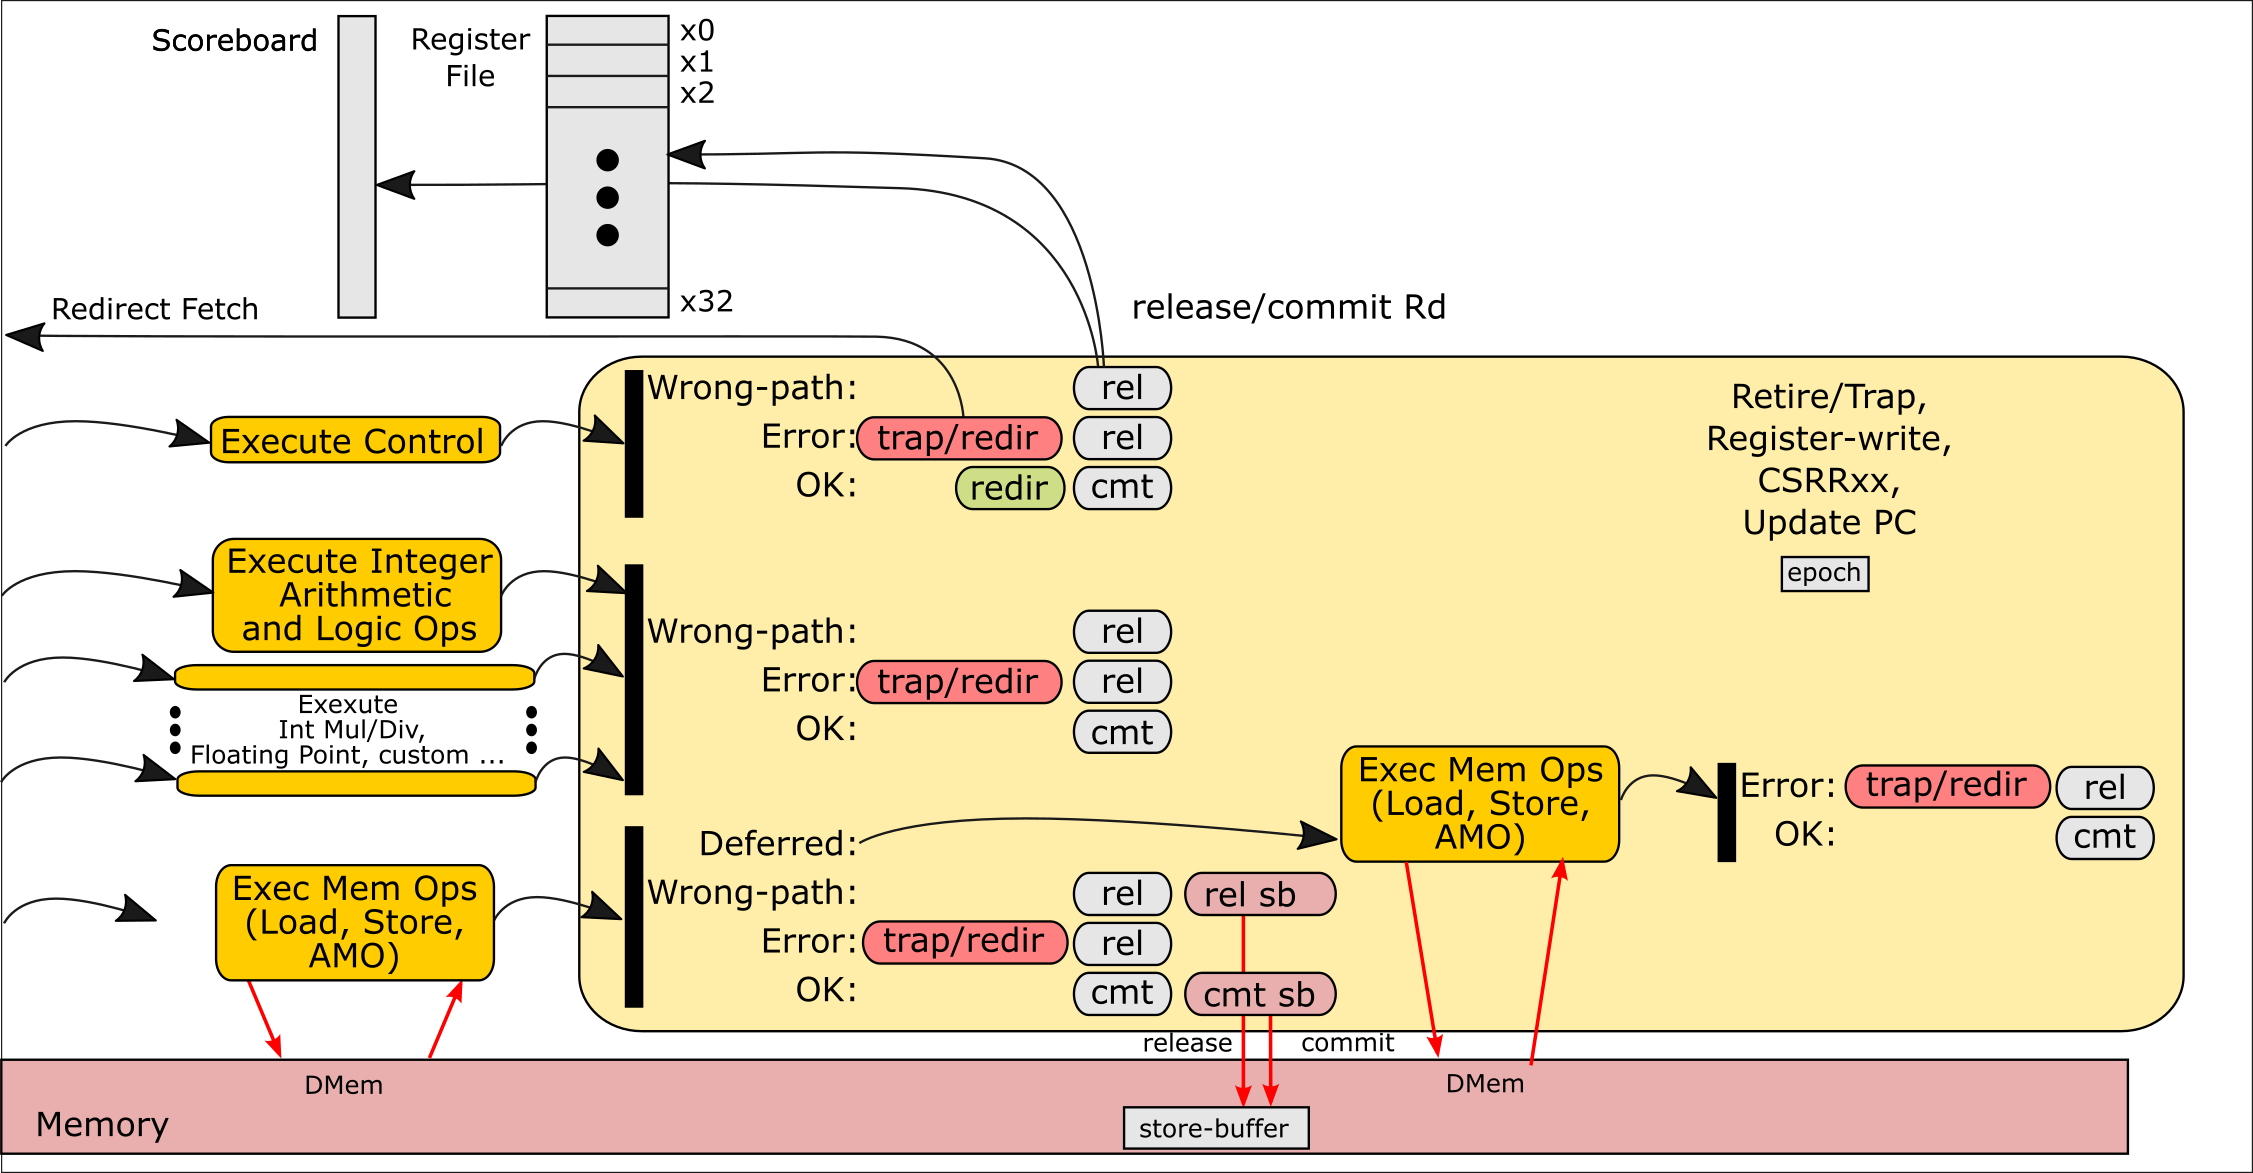
\includegraphics[width=6in,angle=0]{Figures/Fig_Fife_Retire}}
  \caption{\label{Fig_Fife_Retire_2}
           Actions in the ``Retire'' stage of Fife
	   (same as Fig.~\ref{Fig_Fife_Retire})}
\end{figure}

Here is the interface definition for this module:

{\small
\begin{Verbatim}[frame=single, numbers=left, label=(In file:src\_Fife/S5\_Retire.bsv)]
interface Retire_IFC;
   method Action init (Initial_Params initial_params);

   // Forward in
   interface FIFOF_I #(RR_to_Retire)       fi_RR_to_Retire;
   interface FIFOF_I #(Control_to_Retire)  fi_Control_to_Retire;
   interface FIFOF_I #(EX_to_Retire)       fi_IALU_to_Retire;

   // Speculative DMem response and commit/discard
   interface FIFOF_I #(Mem_Rsp)                fi_DMem_S_rsp;
   interface FIFOF_O #(Retire_to_DMem_Commit)  fo_DMem_S_commit;

   // Non-speculative DMem
   interface FIFOF_O #(Mem_Req)  fo_DMem_req;
   interface FIFOF_I #(Mem_Rsp)  fi_DMem_rsp;

   // Backward out
   interface FIFOF_O #(F_from_Retire)      fo_F_from_Retire;
   interface FIFOF_O #(RW_from_Retire)     fo_RW_from_Retire;
endinterface
\end{Verbatim}
}

The first four \verb|fi_XXX| sub-interfaces correspond to the black
arrows entering the Retire module from the left in the figure.  The
next two \verb|fo_XXX| sub-interfaces correspond to the outgoing red
arrows at the bottom of the module, and the next sub-interface
(\verb|fi_DMem_rsp|) is the incoming red arrow at the bottom of the
module returning a non-speculative memory response.  The last two
sub-interfaces are the black output arrows at the top of the module
carrying redirections to the Fetch stage and Register-Writes to the
\verb|RR_RW| module, respectively.

We define a ``state'' for this module:

{\small
\begin{Verbatim}[frame=single, numbers=left, label=(In file:src\_Fife/S5\_Retire.bsv)]
typedef enum {STATE_PIPE,        // Normal pipeline operation
	      STATE_DMEM_RSP     // Handle Non-speculative DMem response
} Module_State
deriving (Bits, Eq, FShow);
\end{Verbatim}
}

Normally the module is in \verb|STATE_PIPE|, acting as the last stage
of the pipeline.  However, in certain circumstances we switch into
non-pipelined ``FSM'' mode, similar to Drum:

\begin{tightlist}

\item to execute non-speculative DMem ops (MMIO/non-memory-like),

\item to execute traps and interrupts (discussed in a later chapter), and

\item to execute CSRRx insructions  (discussed in a later chapter).

\end{tightlist}

Here we see the code for the \verb|mkRetire| module, the Retire stage
(we have elided the BEHAVIOR section which will be discussed shortly).

{\small
\begin{Verbatim}[frame=single, numbers=left, label=(In file:src\_Fife/S5\_Retire.bsv)]
(* synthesize *)
module mkRetire (Retire_IFC);
   // For managing speculation, redirection traps, etc.
   Reg #(Epoch) rg_epoch  <- mkReg (0);

   // Forward in
   // Depth of f_RR_to_Retire should be > longest EX pipe
   FIFOF #(RR_to_Retire)       f_RR_to_Retire      <- mkSizedFIFOF (8);
   FIFOF #(Control_to_Retire)  f_Control_to_Retire <- mkPipelineFIFOF;
   FIFOF #(EX_to_Retire)       f_IALU_to_Retire    <- mkPipelineFIFOF;
   FIFOF #(Mem_Rsp)            f_DMem_S_rsp        <- mkPipelineFIFOF;

   // Forward out
   FIFOF #(Retire_to_DMem_Commit) f_DMem_S_commit  <- mkBypassFIFOF;

   // Backward out
   FIFOF #(F_from_Retire)   f_F_from_Retire  <- mkBypassFIFOF;
   FIFOF #(RW_from_Retire)  f_RW_from_Retire <- mkBypassFIFOF;

   // Non-speculative DMem reqs and rsps
   FIFOF #(Mem_Req)  f_DMem_req  <- mkBypassFIFOF;
   FIFOF #(Mem_Rsp)  f_DMem_rsp  <- mkPipelineFIFOF;

   Reg #(Module_State) rg_state <- mkReg (STATE_PIPE);

   // ================================================================
   // BEHAVIOR

   ... to be discussed shortly ...

   // ================================================================
   // INTERFACE

   method Action init (Initial_Params initial_params);
      ...
   endmethod

   // Forward in
   interface fi_RR_to_Retire      = to_FIFOF_I (f_RR_to_Retire);
   interface fi_Control_to_Retire = to_FIFOF_I (f_Control_to_Retire);
   interface fi_IALU_to_Retire    = to_FIFOF_I (f_IALU_to_Retire);

   // Speculative DMem
   interface fi_DMem_S_rsp        = to_FIFOF_I (f_DMem_S_rsp);
   interface fo_DMem_S_commit     = to_FIFOF_O (f_DMem_S_commit);

   // Non-speculative DMem
   interface fo_DMem_req       = to_FIFOF_O (f_DMem_req);
   interface fi_DMem_rsp       = to_FIFOF_I (f_DMem_rsp);

   // Backward out
   interface fo_F_from_Retire  = to_FIFOF_O (f_F_from_Retire);
   interface fo_RW_from_Retire = to_FIFOF_O (f_RW_from_Retire);
endmodule
\end{Verbatim}
}

The first section (preceding BEHAVIOR) instantiates register
\verb|rg_epoch| to keep track of the epoch, and then FIFOs for all the
incoming and outgoing channels.  Finally, it instantiates register
\verb|rg_state| to hold the current module state.

The final, INTERFACE, section, as before, has an \verb|init| method,
and then lifts the various FIFO interfaces into sub-interfaces for
this module.

The BEHAVIOR section consists of a collection of rules, each handling
a distinct scenario.  In overview:

\begin{itemize}

  \item Rule \verb|rl_Retire_wrong_path| handles all mis-predicted
        instructions.

  \item Rules \verb|rl_Retire_normal| and \verb|rl_Retire_exc| handle
        instructions with \verb|EXEC_TAG_RETIRE|, {\ie} instructions
        that only have a direct message from the
        Register-Read-and-Dispatch stage, with nothing in any of the
        other execution pipelines.

  \item Rules \verb|rl_Retire_Control_normal| and
        \verb|rl_Retire_Control_exc| handle instructions with
        \verb|EXEC_TAG_CONTROL|, {\ie} BRANCH and JAL/JALR
        instructions that came through the Execute Control pipe.

  \item Rules \verb|rl_Retire_Int_normal| and \verb|rl_Retire_Int_exc|
        handle instructions with \verb|EXEC_TAG_INT|---LUI, AUIPC and
        Integer Arithmetic/Logic instructions that came through the
        Execute Int pipe.

  \item Rules \verb|rl_Retire_DMem_S_normal| and
        \verb|rl_Retire_DMem_S_exc| handle instructions with
        \verb|EXEC_TAG_DMEM|---LOAD and STORE instructions that came
        through the Execute DMem pipe---and were executed
        speculatively (into memory-like addresses).

  \item Rules \verb|rl_Retire_DMem_deferred| and
        \verb|rl_Retire_DMem_rsp| handle instructions with
        \verb|EXEC_TAG_DMEM|---LOAD and STORE instructions that came
        through the Execute DMem pipe---and were deferred (not
        executed) because they were for MMIO/non-memory-like addresses.

\end{itemize}

Each pair of rules \verb|rl_XXX_normal| and \verb|rl_XXX_exc| handle
the two cases where the instruction completes normally {\vs} the
instruction has raised an exception (trap).

% ================================================================

\subsection{Common facilities used by many rules}

\label{Sec_Retire_Common}

The following function captures the actions to be taken when we
discover that the prediction for the successor to this instruction was
wrong.  The boolean \verb|mispredicted| indicates whether the
prediction was correct or not.  If the prediction was correct, no
action is taken.  Otherwise, we increment the epoch, and send a
redirection message to the Fetch stage with the correct PC and the new
epoch.  The disposition of this message was discussed in
Section~\ref{Sec_Fife_Fetch_stage}.

{\small
\begin{Verbatim}[frame=single, numbers=left, label=(In file:src\_Fife/S5\_Retire.bsv)]
   // Redirect Fetch stage on mispredicted PC
   function Action fa_redirect_Fetch (Bool         mispredicted,
				      RR_to_Retire x1,
				      Bit #(XLEN)  next_pc);
      action
	 if (mispredicted) begin
	    let next_epoch = rg_epoch + 1;
	    rg_epoch <= next_epoch;
	    let y = F_from_Retire {inum:       x1.inum,
				   pc:         x1.pc,
				   instr:      x1.instr,
				   next_pc:    next_pc,
				   next_epoch: next_epoch};
	    f_F_from_Retire.enq (y);
	 end
      endaction
   endfunction
\end{Verbatim}
}

The following function captures the actions to be taken for updating
an instruction's destination rd register.  It simply assembles a
\verb|RW_to_Retire| message and sends it to the \verb|RR_RW| module.
The disposition of this message was discussed in
Section~\ref{Sec_RR_RW_module}.

{\small
\begin{Verbatim}[frame=single, numbers=left, label=(In file:src\_Fife/S5\_Retire.bsv)]
   // Update Rd for those instructions that have an Rd 
   function Action fa_update_rd (RR_to_Retire x1, Bool commit, Bit #(XLEN) rd_val);
      action
	 let y = RW_from_Retire {inum:       x1.inum,
				 pc:         x1.pc,
				 instr:      x1.instr,
				 rd:         instr_rd (x1.instr),
				 commit:     commit,
				 data:       rd_val};
	 f_RW_from_Retire.enq (y);
      endaction
   endfunction
\end{Verbatim}
}

The following definitions examine the first element of the
\verb|f_RR_to_Retire| (direct path) queue, which controls how incoming
instructions are merged and disposed of, in the rules that follow.

{\small
\begin{Verbatim}[frame=single, numbers=left, label=(In file:src\_Fife/S5\_Retire.bsv)]
   RR_to_Retire x_rr_to_retire = f_RR_to_Retire.first;

   Bool wrong_path = (x_rr_to_retire.epoch != rg_epoch);
   Bool is_Direct  = (x_rr_to_retire.exec_tag == EXEC_TAG_RETIRE);
   Bool is_Control = (x_rr_to_retire.exec_tag == EXEC_TAG_CONTROL);
   Bool is_Int     = (x_rr_to_retire.exec_tag == EXEC_TAG_IALU);
   Bool is_DMem    = (x_rr_to_retire.exec_tag == EXEC_TAG_DMEM);
\end{Verbatim}
}

The incoming instruction is a wrong-path instruction if its
accompanying epoch does not match our \verb|rg_epoch| register.  The
remaining four definitions summarize the class of the instruction
based on the execution tag; these control which of the following rules
will fire.

% ================================================================

\subsection{Rule to discard wrong-path instructions}

For a wrong-path instruction, we must dequeue it from
\verb|f_RR_to_Retire| and any associated Execute queue (Control, Int
or DMem).  It if is a DMem STORE instruction that was performed
speculatively, we must also send a ``discard'' message to the head of
the store-buffer.  Finally, if the instruction has an rd destination
register, we must send an discard-scoreboard-reservation message to
the RR-RW module using the \verb|fa_update_rd| function described in
the Section~\ref{Sec_Retire_Common}.

{\small
\begin{Verbatim}[frame=single, numbers=left, label=(In file:src\_Fife/S5\_Retire.bsv)]
   rule rl_Retire_wrong_path ((rg_state == STATE_PIPE)
			      && wrong_path);
      f_RR_to_Retire.deq;

      if (is_Control) f_Control_to_Retire.deq;
      if (is_Int)     f_IALU_to_Retire.deq;
      if (is_DMem) begin
	 f_DMem_S_rsp.deq;

	 // Send discard to Store Buffer, if needed
	 Bool commit_store_val = ((! is_LOAD (x_rr_to_retire.instr))
				  && (! is_LR (x_rr_to_retire.instr))
				  && (f_DMem_S_rsp.first.rsp_type == MEM_RSP_OK));
	 if (commit_store_val) begin
	    let y = Retire_to_DMem_Commit{inum:   x_rr_to_retire.inum,
					  commit: False};
	    f_DMem_S_commit.enq (y);
	 end
      end

      // Release rd scoreboard reservation, if has one
      Bool rd_commit = False;
      if (x_rr_to_retire.has_rd) fa_update_rd (x_rr_to_retire, rd_commit, ?);
   endrule
\end{Verbatim}
}

% ================================================================

\subsection{Rules to retire instructions direct from RR-RW}

The following rules handle instructions that are direct from the RR-RW
stage, {\ie} which were \emph{not} also sent through any of the
Execute pipes (Control, Int or DMem).

If it is not an exception, then it must be a CSRRx instruction, which
we have not yet implemented yet (we will do so in
Chapter~\ref{ch_Fife_Exception}).  For now, we treat it as a no-op.  We
dequeue the instruction from \verb|f_RR_to_Retire|.  For CSRRx
instructions, the correct next-PC is the fall-through PC, so we check
this against the predicted PC, and redirect if necessary using
action-function \verb|fa_redirect_fetch()| which was described in
Section~\ref{Sec_Retire_Common}.

{\small
\begin{Verbatim}[frame=single, numbers=left, label=(In file:src\_Fife/S5\_Retire.bsv)]
   rule rl_Retire_normal ((rg_state == STATE_PIPE)
                          && (! wrong_path)
                          && is_Direct
			  && (! x_rr_to_retire.exception));
      f_RR_to_Retire.deq;

      $display ("CSRRx instructions not yet implemented; no-op for now");

      // Redirect Fetch PC if mispredicted
      Bool mispredicted = (x_rr_to_retire.predicted_pc
                           != x_rr_to_retire.fallthru_pc);
      fa_redirect_Fetch (mispredicted, x_rr_to_retire, x_rr_to_retire.fallthru_pc);
   endrule
\end{Verbatim}
}

If the first element of \verb|f_RR_to_Retire| is carrying an
exception, this could be due to a memory-fault during Fetch, or
detection of an illegal instruction during Decode.  In
Chapter~\ref{ch_Fife_Exception} we will describe how to handle
exceptions, but for now we use \verb|$finish()| to abort the
simulation.

{\small
\begin{Verbatim}[frame=single, numbers=left, label=(In file:src\_Fife/S5\_Retire.bsv)]
   rule rl_Retire_exc ((rg_state == STATE_PIPE)
                       && (! wrong_path)
		       && is_Direct
		       && x_rr_to_retire.exception);
      f_RR_to_Retire.deq;

      $display ("Exception-handling not yet implemented");
      $finish (1);
   endrule
\end{Verbatim}
}

% ================================================================

\subsection{Rules to retire instructions from the Execute Control path}

If the instruction is a Control instruction without an exception, we
pop the relevant incoming queues (\verb|f_RR_to_Retire| and
\verb|f_Control_to_Retire|), update the Rd destination register (JAL
and JALR often save a ``return address'' in rd), and redirect the
Fetch stage if mispredicted.

{\small
\begin{Verbatim}[frame=single, numbers=left, label=(In file:src\_Fife/S5\_Retire.bsv)]
   rule rl_Retire_Control_normal ((rg_state == STATE_PIPE)
                                  && (! wrong_path)
				  && is_Control
				  && (! f_Control_to_Retire.first.exception));
      f_RR_to_Retire.deq;
      let x2 <- pop_o (to_FIFOF_O (f_Control_to_Retire));

      // Updata rd if valid
      Bool rd_commit = True;
      if (x2.data_valid) fa_update_rd (x_rr_to_retire, rd_commit, x2.data);

      // Redirect Fetch PC if mispredicted
      Bool mispredicted = (x_rr_to_retire.predicted_pc != x2.next_pc);
      fa_redirect_Fetch (mispredicted,  x_rr_to_retire, x2.next_pc);
   endrule
\end{Verbatim}
}

If the instruction is carrying an exception this is because the
BRANCH, JAL or JALR target was misaligned.  In
Chapter~\ref{ch_Fife_Exception} we will describe how to handle
exceptions, but for now we use \verb|$finish()| to abort the
simulation.

{\small
\begin{Verbatim}[frame=single, numbers=left, label=(In file:src\_Fife/S5\_Retire.bsv)]
   rule rl_Retire_Control_exc ((rg_state == STATE_PIPE)
                               && (! wrong_path)
                               && is_Control
			       && f_Control_to_Retire.first.exception);
      f_RR_to_Retire.deq;
      let x2 <- pop_o (to_FIFOF_O (f_Control_to_Retire));

      $display ("Exception-handling not yet implemented");
      $finish (1);
   endrule
\end{Verbatim}
}

% ================================================================

\subsection{Rules to retire instructions from the Execute Int path}

The two rules to retire instructions from the Execute Int path are
similar to the rules for the Control path in the previous section.

If the instruction is without an exception, we pop the relevant
incoming queues (\verb|f_RR_to_Retire| and \verb|f_IALU_to_Retire|),
update the Rd destination register, and redirect the Fetch stage if
mispredicted.

{\small
\begin{Verbatim}[frame=single, numbers=left, label=(In file:src\_Fife/S5\_Retire.bsv)]
   rule rl_Retire_Int_normal ((rg_state == STATE_PIPE)
			      && (! wrong_path)
			      && is_Int
			      && (! f_IALU_to_Retire.first.exception));
      f_RR_to_Retire.deq;
      EX_to_Retire x2 <- pop_o (to_FIFOF_O (f_IALU_to_Retire));

      // Updata rd if valid
      Bool rd_commit = True;
      if (x2.data_valid) fa_update_rd (x_rr_to_retire, rd_commit, x2.data);

      // Redirect Fetch PC if mispredicted
      Bool mispredicted = (x_rr_to_retire.predicted_pc != x_rr_to_retire.fallthru_pc);
      fa_redirect_Fetch (mispredicted, x_rr_to_retire, x_rr_to_retire.fallthru_pc);
   endrule
\end{Verbatim}
}

If the instruction is carrying an exception: in
Chapter~\ref{ch_Fife_Exception} we will describe how to handle
exceptions, but for now we use \verb|$finish()| to abort the
simulation.

{\small
\begin{Verbatim}[frame=single, numbers=left, label=(In file:src\_Fife/S5\_Retire.bsv)]
   rule rl_Retire_Control_exc ((rg_state == STATE_PIPE)
                               && (! wrong_path)
                               && is_Control
			       && f_Control_to_Retire.first.exception);
      f_RR_to_Retire.deq;
      let x2 <- pop_o (to_FIFOF_O (f_Control_to_Retire));

      $display ("Exception-handling not yet implemented");
      $finish (1);
   endrule
\end{Verbatim}
}

Note, none of the standard RISC-V Integer instructions raise any
exceptions, so we do not expect this rule to ever be
executed. However, if we extend the ISA to new Integer instructions
that could raise an exception, this rule is ready to field those
exceptions.

% ================================================================

\subsection{Rules to retire instructions from the Execute DMem path}

From the Execute DMem path we receive memory responses.  If the
response type is \verb|MEM_RSP_OK| then this instruction was executed
speculatively and successfully; we just have to retire it just like
the Control and Int scenarios above, with the additional need to send
a ``commit'' message to the store-buffer if it wrote to memory.

{\small
\begin{Verbatim}[frame=single, numbers=left, label=(In file:src\_Fife/S5\_Retire.bsv)]
   rule rl_Retire_Dmem_S_normal ((rg_state == STATE_PIPE)
				 && (! wrong_path)
				 && is_DMem
				 && (f_DMem_S_rsp.first.rsp_type == MEM_RSP_OK));
      f_RR_to_Retire.deq;
      let x2 <- pop_o (to_FIFOF_O (f_DMem_S_rsp));

      Bool rd_commit = True;
      if (x_rr_to_retire.has_rd)
	 fa_update_rd (x_rr_to_retire, rd_commit, truncate (x2.data));

      // Send commit to Store Buffer if it wrote to memory
      Bool wrote_mem = ((! is_LOAD (x_rr_to_retire.instr))
		        && (! is_LR (x_rr_to_retire.instr)));
      if (wrote_mem) begin
	 let y = Retire_to_DMem_Commit{inum:   x_rr_to_retire.inum,
				       commit: True};
	 f_DMem_S_commit.enq (y);
      end

      // Redirect Fetch PC if mispredicted
      Bool mispredicted = (x_rr_to_retire.predicted_pc != x_rr_to_retire.fallthru_pc);
      fa_redirect_Fetch (mispredicted, x_rr_to_retire, x_rr_to_retire.fallthru_pc);
   endrule
\end{Verbatim}
}

If the DMem response indicates that it attempted a speculative access
and encountered an exception, the memory response type will be
\verb|MEM_RSP_ERR| or \verb|MEM_RSP_MISALIGNED|.  We compute the
appropriate RISC-V exception \verb|cause| code.  In
Chapter~\ref{ch_Fife_Exception} we will describe how to handle
exceptions, but for now we use \verb|$finish()| to abort the
simulation.

{\small
\begin{Verbatim}[frame=single, numbers=left, label=(In file:src\_Fife/S5\_Retire.bsv)]
   Bool dmem_S_rsp_exception = ((f_DMem_S_rsp.first.rsp_type    == MEM_RSP_ERR)
				|| (f_DMem_S_rsp.first.rsp_type == MEM_RSP_MISALIGNED));

   rule rl_Retire_Dmem_S_exc ((rg_state == STATE_PIPE)
			      && (! wrong_path)
			      && is_DMem
			      && dmem_S_rsp_exception);
      f_RR_to_Retire.deq;
      let x2 <- pop_o (to_FIFOF_O (f_DMem_S_rsp));

      Bit #(XLEN)  cause = ?;
      if (x2.rsp_type == MEM_RSP_MISALIGNED)
	 cause = (is_LOAD (x_rr_to_retire.instr)
		  ? cause_LOAD_ADDRESS_MISALIGNED
		  : cause_STORE_AMO_ADDRESS_MISALIGNED);
      else
	 cause = (is_LOAD (x_rr_to_retire.instr)
		  ? cause_LOAD_ACCESS_FAULT
		  : cause_STORE_AMO_ACCESS_FAULT);

      $display ("Exception-handling not yet implemented");
      $finish (1);
   endrule
\end{Verbatim}
}

If the DMem response indicates that it deferred the request because
the address was to an MMIO/non-memory-like address, the memory
response type will be \verb|MEM_RSP_ERR| or \verb|MEM_REQ_DEFERRED|.
In this case, we now construct the memory response and send it to
memory.  Finally we change the module state to \verb|STATE_DMEM_RSP|
indicating that we will now await the memory response.  Note, this all
previous rules will no longer fire because they all have
``\verb|(rg_state == STATE_PIPE)|'' in their rule conditions, which is
now false.

{\small
\begin{Verbatim}[frame=single, numbers=left, label=(In file:src\_Fife/S5\_Retire.bsv)]
   rule rl_Retire_DMem_deferred ((rg_state == STATE_PIPE)
                                 && (! wrong_path)
				 && is_DMem
				 && (f_DMem_S_rsp.first.rsp_type == MEM_REQ_DEFERRED));
      let x2 <- pop_o (to_FIFOF_O (f_DMem_S_rsp));
      let mem_req = Mem_Req{inum:     x2.inum,
			    pc:       x2.pc,
			    instr:    x2.instr,
			    req_type: x2.req_type,
			    size:     x2.size,
			    addr:     x2.addr,
			    data:     x2.data};
      f_DMem_req.enq (mem_req);
      rg_state <= STATE_DMEM_RSP;
   endrule
\end{Verbatim}
}

The final rule, handles the corresponding responses from memory.  We
pop the direct-path information (\verb|f_RR_to_Retire|) and the
memory-response (\verb|f_DMem_Rsp|).

If the response returned an exception, we compute the RISC-V exception
\verb|cause|.  In Chapter~\ref{ch_Fife_Exception} we will describe how
to handle exceptions, but for now we use \verb|$finish()| to abort the
simulation.

Next we check for \verb|MEM_REQ_DEFERRED| responses.  This is a
redundant check in that it should be impossible---the non-speculative
DMem port should never defer any requests---and is just a bit of
defensive programming in case of a bug in the memory system.  We abort
the simulation with \verb|$finish()|.

On successful responses (\verb|MEM_RSP_OK|) we perform the usual
writeback-register and possible redirection on misprediction.

Finally, we set \verb|rg_state| to \verb|STATE_PIPE|, which once again
enables all the pipeline rules.

{\small
\begin{Verbatim}[frame=single, numbers=left, label=(In file:src\_Fife/S5\_Retire.bsv)]
   rule rl_Retire_DMem_rsp (rg_state == STATE_DMEM_RSP);
      f_RR_to_Retire.deq;
      let mem_rsp <- pop_o (to_FIFOF_O (f_DMem_rsp));

      Bool exception = ((mem_rsp.rsp_type == MEM_RSP_ERR)
			|| (mem_rsp.rsp_type == MEM_RSP_MISALIGNED));
      Bit #(XLEN)  cause = ?;
      if (exception) begin
	 if (mem_rsp.rsp_type == MEM_RSP_MISALIGNED)
	    cause = (is_LOAD (x_rr_to_retire.instr)
		     ? cause_LOAD_ADDRESS_MISALIGNED
		     : cause_STORE_AMO_ADDRESS_MISALIGNED);
	 else
	    cause = (is_LOAD (x_rr_to_retire.instr)
		     ? cause_LOAD_ACCESS_FAULT
		     : cause_STORE_AMO_ACCESS_FAULT);
	 $finish (1);
      end
      else if (mem_rsp.rsp_type == MEM_REQ_DEFERRED) begin
         $display ("IMPOSSIBLE: Unexpected MEM_REQ_DEFERRED; FINISH.");
	 $finish (1);
      end
      else begin
      	 // mem_rsp.rsp_type will be MEM_REQ_OK here

	 // Writeback register
	 Bool rd_commit = True;
	 if (x_rr_to_retire.has_rd)
	    fa_update_rd (x_rr_to_retire, rd_commit, truncate (mem_rsp.data));

	 // Redirect Fetch to correct mispredicted PC
	 fa_redirect_Fetch ((x_rr_to_retire.predicted_pc != x_rr_to_retire.fallthru_pc),
			    x_rr_to_retire,
			    x_rr_to_retire.fallthru_pc);
      end
      // Go back to pipeline behavior
      rg_state <= STATE_PIPE;
   endrule
\end{Verbatim}
}

Note that in this module, when we have a DMem response with
response-type \verb|MEM_REQ_DEFERRED| we effectively switch from
pipeline processing to Drum-like FSM processing (one FSM state issues
a DMem request and another FSM state fields the response and processes
it).  This is a standard trick: for an instruction that cannot for
some reason be pipelined, we execute it completely in the Retire
module in Drum-like FSM mode.  In fact, we shall use exactly this
trick to implement CSRRxx instructions (in
Chapter~\ref{ch_Fife_CSRRxx}, because CSRRx instructions are tricky to
execute in the main pipeline.

% ****************************************************************
